\documentclass[a4paper, 10pt, deutsch]{llncs}

\usepackage{graphicx}
\usepackage{multicol}
\usepackage[bottom]{footmisc}

\usepackage{amsbsy,amscd,amsfonts,amssymb,amstext,amsmath,latexsym,theorem}

\usepackage[T1]{fontenc}

\usepackage[USenglish]{babel}

\usepackage[utf8]{inputenc}

\usepackage{subfigure}

\pagestyle{plain}
\bibliographystyle{unsrt}

%%%%%%%%%%%%%%%%%%%%%%%%%%%%%%%%%%%%%%%%%%%%%%%%%%%%%%%%%%%%%%%%%%%%%

\begin{document}

\title{{\normalsize Visual Computing Lab} \\
  Visualization of the Most Effective Features Extracted by ConvNets for Detection Tasks}
\author{Maximilian Kircher, Advisor: Faraz Saeedan}
\institute{ TU Darmstadt, Visual Inference}

\maketitle

In this lab, the task was, to apply the methods presented in \cite{simonyan2013deep} to the network of \cite{liu2016ssd}.


\section{Class Model Visualization}
\subsection{VGG}

First I tried to reproduce the results from \cite{simonyan2013deep} with a vgg network. As examples I used the category \textit{goose}, as an example of this category is also provided by the paper. (\ref{fig:1} a)\\
The objective of the optimization is, to maximize the score for this categorization network. One na\"ive loss function would therefore be $-score(category)$ (\ref{fig:1} b). One problem is, that the output of the network - i.a. the score - seems to often increase, with the input. Therefore the it is possible, that this loss function leads to chaos (\ref{fig:1} c).
A solution is an additional loss, that can be added to the loss function and ensures, that the values of the image don't become to big: Each pixel is squared and the mean over all pixel values is computed. (short: sq) (\ref{fig:1} d-h)\\
With the combined loss, the methods produces good results, that are comparable to the result of the paper.\\
% lam 1e4
It can be seen, that a learning rate of 1 produces good results, while the results with to high or low learning rates are not that good (\ref{fig:1} g,h).
Another loss function instead of the negative class score, that came to my mind, was $\dfrac{1}{score(category)}$.
But experiments with this function showed, that it seems to be not useful for the task (\ref{fig:1} i-l).

\begin{figure}
\centering
\subfigure[result presented by \cite{simonyan2013deep}]{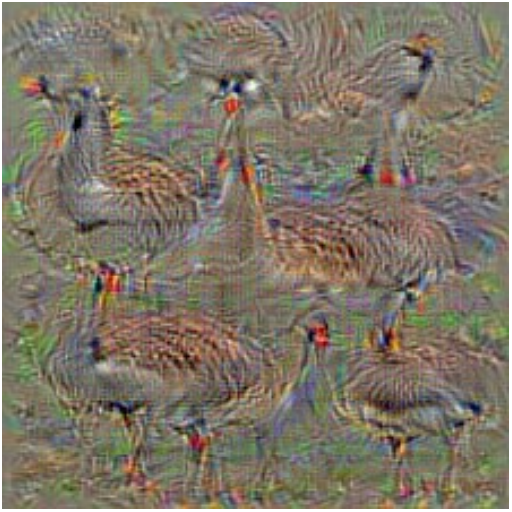
\includegraphics[scale=0.29]{../new/goose_paper.png}}
\subfigure[loss:-sc,lr:1,it:100]{\includegraphics[scale=0.5]{../new/goose_min-l2_100_1,0.png}}
\subfigure[loss:-sc,lr:1,it:500]{\includegraphics[scale=0.5]{../new/goose_min-l2_500_1,0.png}}
\subfigure[loss:-sc+sq,lr:1,it:100]{\includegraphics[scale=0.5]{../new/goose_min_100_1,0.png}}
\subfigure[loss:-sc+sq,lr:1,it:500]{\includegraphics[scale=0.5]{../new/goose_min_500_1,0.png}}
\subfigure[loss:-sc+sq,lr:1,it:1000]{\includegraphics[scale=0.5]{../new/goose_min_1000_1,0.png}}
\subfigure[loss:-sc+sq,lr:5,it:500]{
\includegraphics[scale=0.5]{../new/goose_min_500_5.png}}
\subfigure[loss:-sc+sq,lr:0.1,it:500]{\includegraphics[scale=0.5]{../new/goose_min_500_0,1.png}}
\subfigure[loss:1/sc,lr:1,it:100]{\includegraphics[scale=0.5]{../new/goose_div-l2_100_1,0.png}}
\subfigure[loss:1/sc,lr:5,it:500]{\includegraphics[scale=0.5]{../new/goose_div-l2_500_5,0.png}}
\subfigure[loss:1/sc+sq,lr:5,it:500]{\includegraphics[scale=0.5]{../new/goose_div_500_5,0.png}}
\subfigure[loss:1/sc+sq,lr:1,it:1000]{\includegraphics[scale=0.5]{../new/goose_div_1000_1,0.png}}
\caption{Results of the class model visualization a vgg network for the category goose. lr is the used learning rate, it the number of iterations}
\label{fig:1}
\end{figure}


\subsection{SSD}

For this network I chose the category \textit{horse}, as the implementation I used was trained for other categories, than the 1000 image net categories.\\
As the ssd network is an object detection network and no categorization network, the loss function, that I used for the vgg network, can not be used directly here.
There are different so called prior boxes used in the network, that determine, where it looks for the objects. When I tried to use the biggest of them and maximize the category score as for the vgg network and added an additional term, that should ensure, that the prediction for this box is localized at the whole image, it produced bad results. Also it can be seen, that it still concentrates on the upper left part.\\
The second loss function I tried was, to maximize the category score for all prior box prediction. In the result, can be seen, that there are very many little structures, that might be horses, but that are not that clear.\\
Third I used the criterion, that was also used, when training the network. It computes an localization and an confidence loss for a given target, for which I chose the wanted category and as boundaries the whole image. This loss produced the best results.\\
This loss I used, to visualize a smaller (1/4) object at the center of the image. There are no big differences to the bigger version...


\section{Image-Specific Class Saliency Visualisation}
\label{sec:1}





\bibliography{bibliography}


\end{document}





